\section{Methodology}

\subsection{Overview of the Emperor Penguin Optimizer Algorithm}

The algorithm represents a population of potential solutions as a colony of penguins, where each penguin's position corresponds to a potential solution to the optimization problem. 

It iteratively updates the positions of the penguins on the basis of the temperature profile and the distance among them. 
Initially, the population of emperor penguins is randomly positioned. 
The fitness of each penguin is then evaluated to determine how well they solve the optimization problem. 
During each iteration, a huddling boundary is created, and the temperature profile is evaluated. 
Based on this profile, the penguins are relocated and for each penguin, the distance to the best penguin is calculated. The positions of the penguins are updated accordingly, 
and their fitness is re-evaluated. This process continues until a termination criterion is met, 
such as reaching a maximum number of iterations or achieving a satisfactory fitness level. The best solution found during the iterations is returned as the final result. 

We report the original implementation of the algorithm in pseudocode, followed by our implementation of the algorithm.

\begin{algorithm}[H]
    \caption{Emperor Penguin Optimizer (EPO)}
    \label{alg:epo}
    \begin{algorithmic}[1]
    \Require Objective function $f(\mathbf{x})$, population size $N$, maximum iterations $Max_{\text{iter}}$, huddle radius $R$, movement parameters $M$, exploration parameters $f$, exploitation parameters $l$
    
    \State Initialize population of penguins $\vec{P_i}$ $(i = 1, 2, \dots, N)$ randomly

    \State $\vec{P_{\text{best}}} \gets \underset{i}{\arg\min} f(\vec{P_i})$ \Comment{Initialize the best solution}
    
    \While {$itr < Max_{\text{iter}}$}
        \State $R \gets Rand(0, 1)$ \Comment{Random number in the range $[0, 1]$}
        
        \If {$R > 1$}
            \State $T \gets 0$
        \Else
            \State $T \gets 1$
        \EndIf

        \State $T' \gets (T - \frac{Max_{\text{iter}}}{itr - Max_{\text{iter}}})$ \Comment{Compute the temperature profile}

        \State $S \gets \Bigl(\sqrt{f\cdot\exp^{-itr/l}-\exp{-itr}}\Bigr)^2$ \Comment{Compute the social force}

        \For {$i = 1$ to $N$}
            \State $\vec{C} \gets Rand(0, 1)$ \Comment{Generate the avoidance vector}
            
            \State $\vec{A} \gets (M \cdot (T' + |\vec{P_{\text{best}}} - \vec{P_i}|)) \cdot R - T'$ \Comment{Compute the movement vector}

            \State $\vec{D} \gets |S \cdot \vec{P_i} - \vec{C} \cdot \vec{P_{\text{best}}}|$ \Comment{Compute the distance vector}

            \State $\vec{P_i} \gets \vec{P_{\text{best}}} - \vec{A} \cdot \vec{D}$ \Comment{Update the position of the penguin}
            \State Clamp $\vec{P_i}$ to the search space bounds
        \EndFor

        \If {$\underset{i}{\min} f(\vec{P_i}) < f(\vec{P_{\text{best}}})$} \Comment{If a better solution is found}

            \State $\vec{P_{\text{best}}} \gets \underset{i}{\arg\min} f(\vec{P_i})$ \Comment{Update the best solution}
        \EndIf

        \State $i \gets i + 1$
    \EndWhile
  
    \State \Return $\vec{P_{\text{best}}}$

    \end{algorithmic}
\end{algorithm}



\subsection{Our Implementation}

Due to the lack of a detailed formalization of the problem, we based our implementation on the works of \cite{EPOWIV} and \cite{rosa2019opytimizer}.\\
We introduced two key changes to the original update rule for the penguin's position. The first modification was the addition of a scaling factor $\alpha \in (0,1]$ to the update rule. This adjustment was necessary because the original algorithm frequently overshot the search space bounds. The second modification involved introducing $\vec{RD}$, a random vector in the range $[-1,1]$, to distribute the penguins more evenly across the search space. This was required as the original algorithm tended to cluster the penguins in the lower-left corner of the search space.

With these modifications, the update rule for the penguin's position becomes:

$$ \vec{P_i} \gets \vec{P_{\text{best}}} - \vec{A} \cdot \vec{D} \cdot \vec{RD} \cdot \alpha $$

% \textbf{TODO:} Consider removing the following pseudocode since the only change is the previous formula.

% \begin{algorithm}[H]
%     \caption{Modified Emperor Penguin Optimizer (mEPO)}
%     \label{alg:ourepo}
%     \begin{algorithmic}[1]
%     \Require Objective function $f(\mathbf{x})$, population size $N$, maximum iterations $Max_{\text{iter}}$, huddle radius $R$, movement parameters $M$, exploration parameters $f$, exploitation parameters $l$, scaling factor $\alpha$
    
%     \State Initialize population of penguins $\vec{P_i}$ $(i = 1, 2, \dots, N)$ randomly

%     \State $\vec{P_{\text{best}}} \gets \underset{i}{\arg\min} f(\vec{P_i})$ \Comment{Initialize the best solution}
    
%     \While {$itr < Max_{\text{iter}}$}
%         \State $R \gets Rand(0, 1)$ \Comment{Random number in the range $[0, 1]$}
        
%         \If {$R > 1$}
%             \State $T \gets 0$
%         \Else
%             \State $T \gets 1$
%         \EndIf

%         \State $T' \gets (T - \frac{Max_{\text{iter}}}{itr - Max_{\text{iter}}})$ \Comment{Compute the temperature profile}

%         \State $S \gets \Bigl(\sqrt{f\cdot\exp^{-itr/l}-\exp{-itr}}\Bigr)^2$ \Comment{Compute the social force}

%         \For {$i = 1$ to $N$}
%             \State $\vec{C} \gets Rand(0, 1)$ \Comment{Generate the avoidance vector}
            
%             \State $\vec{A} \gets (M \cdot (T' + |\vec{P_{\text{best}}} - \vec{P_i}|)) \cdot R - T'$ \Comment{Compute the movement vector}

%             \State $\vec{D} \gets |S \cdot \vec{P_i} - \vec{C} \cdot \vec{P_{\text{best}}}|$ \Comment{Compute the distance vector}

%             \State $\vec{RD} \gets Rand(-1, 1)$ \Comment{Generate a random vector in the range $[-1, 1]$}
            
%             \State $\vec{P_i} \gets \vec{P_{\text{best}}} - \vec{A} \cdot \vec{D} \cdot \vec{RD} \cdot \alpha$
%             \Comment{Update the position of the penguin}
            
%             \State Clamp $\vec{P_i}$ to the search space bounds
%         \EndFor

%         \If {$\underset{i}{\min} f(\vec{P_i}) < f(\vec{P_{\text{best}}})$} \Comment{If a better solution is found}

%             \State $\vec{P_{\text{best}}} \gets \underset{i}{\arg\min} f(\vec{P_i})$ \Comment{Update the best solution}
%         \EndIf

%         \State $i \gets i + 1$
%     \EndWhile
  
%     \State \Return $\vec{P_{\text{best}}}$

%     \end{algorithmic}
% \end{algorithm}

\subsection{Benchmark Test Functions}
After developing our implementation of the algorithm, it was essential to evaluate its accuracy. To achieve this, we used a set of well-known benchmark functions \cite{simulationlib}, each representing varying levels of complexity.
\subsubsection{Sphere Function}

\begin{figure}[H]
    \centering
    \begin{minipage}{0.65\textwidth}
        \begin{equation}
            f(x) = \sum_{i=1}^{n} x_i^2
        \end{equation}
        \textbf{Domain:} \( x_i \in [-5.12, 5.12] \) for all \( i \). \\
        \textbf{Global Optimum:} \( f(x^*) = 0 \) at \( x^* = (0,0,...,0) \).
    \end{minipage}
    \hfill
    \begin{minipage}{0.3\textwidth}
        \centering
        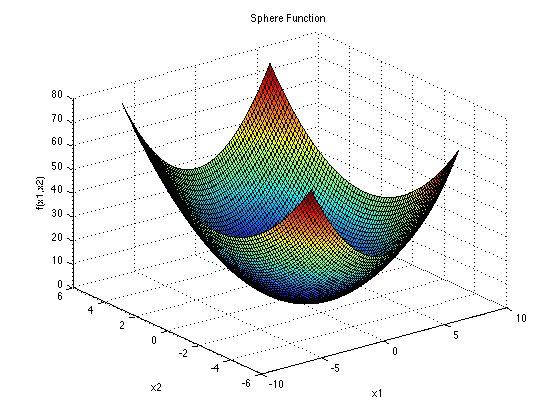
\includegraphics[width=\textwidth]{figures/sphere_function.png}
        \label{fig:sphere}
    \end{minipage}
\end{figure}

\subsubsection{Matyas Function}

\begin{figure}[H]
    \centering
    \begin{minipage}{0.65\textwidth}
        \begin{equation}
            f(x, y) = 0.26(x^2 + y^2) - 0.48xy
        \end{equation}
        \textbf{Domain:} \( x, y \in [-10, 10] \). \\
        \textbf{Global Optimum:} \( f(0,0) = 0 \).
    \end{minipage}
    \hfill
    \begin{minipage}{0.3\textwidth}
        \centering
        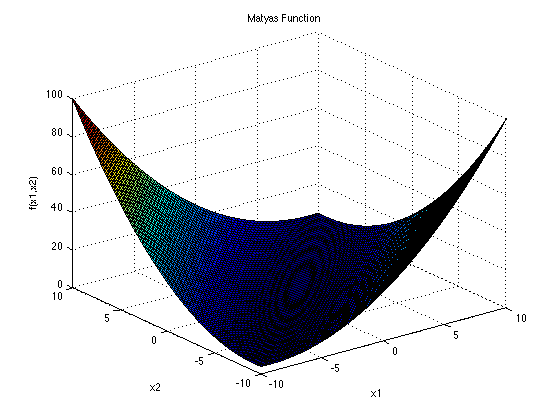
\includegraphics[width=\textwidth]{figures/matyas_function.png}
        \label{fig:matyas}
    \end{minipage}
\end{figure}

\subsubsection{Bukin N.6 Function}

\begin{figure}[H]
    \centering
    \begin{minipage}{0.65\textwidth}
        \begin{equation}
            f(x, y) = 100 \sqrt{|y - 0.01x^2|} + 0.01 |x + 10|
        \end{equation}
        \textbf{Domain:} \( x \in [-15, -5], y \in [-3, 3] \). \\
        \textbf{Global Optimum:} \( f(-10,1) = 0 \).
    \end{minipage}
    \hfill
    \begin{minipage}{0.3\textwidth}
        \centering
        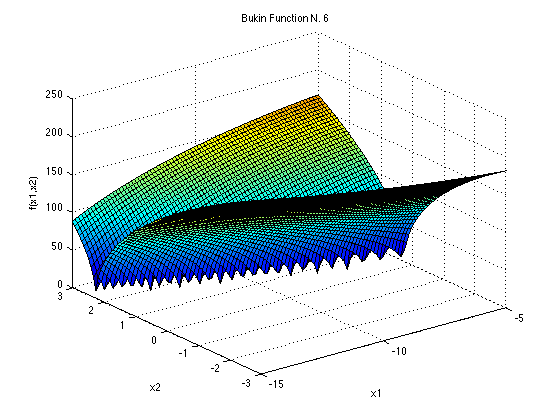
\includegraphics[width=\textwidth]{figures/bukin_function.png}
        \label{fig:bukin}
    \end{minipage}
\end{figure}

\subsubsection{McCormick Function}

\begin{figure}[H]
    \centering
    \begin{minipage}{0.65\textwidth}
        \begin{equation}
            f(x, y) = \sin(x + y) + (x - y)^2 - 1.5x + 2.5y + 1
        \end{equation}
        \textbf{Domain:} \( x \in [-1.5, 4], y \in [-3, 4] \). \\
        \textbf{Global Optimum:} \( f(-0.547, -1.547) = -1.913 \).
    \end{minipage}
    \hfill
    \begin{minipage}{0.3\textwidth}
        \centering
        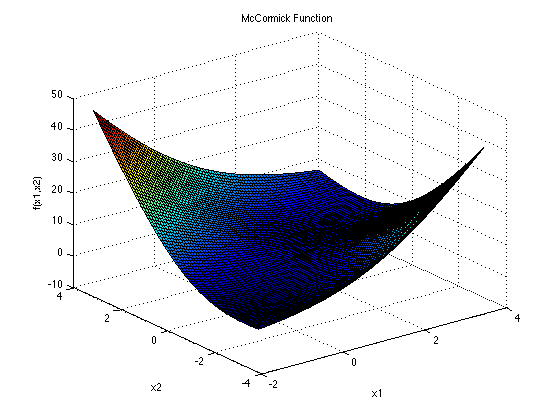
\includegraphics[width=\textwidth]{figures/mccormick_function.png}
    \end{minipage}
\end{figure}

\subsubsection{Michalewicz Function}

\begin{figure}[H]
    \centering
    \begin{minipage}{0.65\textwidth}
        The Michalewicz function is a highly deceptive multimodal function with multiple local minima, making it challenging for optimization algorithms.
        
        \begin{equation}
            f(x) = -\sum_{i=1}^{n} \sin(x_i) \left(\sin\left(\frac{i x_i^2}{\pi}\right)\right)^{2m}
        \end{equation}
        where \( m \) controls the steepness of the valleys and is typically set to \( m = 10 \).

        \textbf{Domain:} \( x_i \in [0, \pi] \) for all \( i \). \\
        \textbf{Global Optimum:} Depends on \( n \), e.g., for \( n = 2 \), \( f(2.20, 1.57) \approx -1.801 \).
    \end{minipage}
    \hfill
    \begin{minipage}{0.3\textwidth}
        \centering
        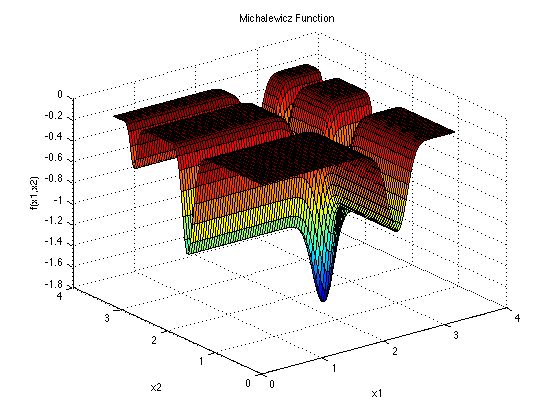
\includegraphics[width=\textwidth]{figures/michalewicz_function.png}
        \label{fig:michalewicz}
    \end{minipage}
\end{figure}


\subsection{Parallelization Strategy}
Like most population-based metaheuristic algorithms, the Emperor Penguin Optimizer (EPO) has
high computational complexity. The search for the optimal solution runs for \( n \) iterations, during which both movement and fitness evaluation are performed for each of the \( p \) penguins in \(m\) variables. Consequently, the overall complexity of the algorithm is \( O(n*p*m) \).
This computational cost is prohibitive for real-world applications, especially when dealing with large-scale problems. To improve feasibility, parallelizing the algorithm could significantly reduce execution time by distributing computations across multiple processors, making it more efficient for complex optimization tasks.
Since the position updates for each penguin are independent and the only information needed is the position of the current best penguin, the algorithm is well-suited for parallelization.
\newline
Our parallelization strategy consists of dividing the population of penguins into $n$ sub-populations, where each sub-population is processed by a different node in the cluster. 
The nodes communicate with each other to share information about the best solution found so far.
Additionally, within each node, the penguin position updates are executed using multithreaded parallelization.
More specifically, at the beginning of the simulation Node 0 sends the simulation parameters (population size, number of iterations, optimization problem, etc.) and broadcasts them to all nodes using \texttt{MPI\_Bcast()}
\newline
At each iteration:
\begin{enumerate}
    \item Each node independently updates the positions of its assigned penguins.
    \item Each node identifies its best local solution.
    \item All nodes use \texttt{MPI\_Allreduce()} to exchange local best values and determine the global best solution.
    \item If the new global best is better than the previous best, the position of the best penguin is broadcasted.
\end{enumerate}

\begin{algorithm}
\caption{PEPO Communication}
\begin{algorithmic}[1]
\Procedure{MPI PEPO}{}
    \State \textbf{Initialize} MPI environment and get $rank$
    \If{$rank = 0$}
        \State Broadcast initial parameters to all processes
    \EndIf
    
    \For{$iteration = 1$ to $maxIterations$}
        \State Update local penguin positions
        \State Calculate local best solution 
        \State \textbf{MPI\_Allreduce}($localBest$, $globalBest$, $MPI\_MINLOC$)
        
        \If{$globalBest.fitness$ < $currentBest.fitness$}
            \State \textbf{MPI\_Bcast}($bestPosition$, $root$=$globalBest.rank$)
            \State Update global best solution
        \EndIf
    \EndFor
\EndProcedure
\end{algorithmic}
\end{algorithm}

Within each node, penguins position updates are further parallelized using \textbf{OpenMP}.
Specifically, \texttt{omp parallel for} is used with dynamic scheduling to parallelize the main loop that updates each penguin's position. The implementation creates dynamic thread-local arrays ($P\_grid$, $A$, and $D\_ep$) to avoid race conditions when calculating position updates.
The parallelization scope includes the entire position update process.
